\documentclass[conference]{IEEEtran}
\usepackage{graphicx}
\usepackage{graphics}
\usepackage{amsmath}
\usepackage[spanish, english]{babel}
\usepackage{hyperref}
\usepackage{float}
\def\BibTeX{{\rm B\kern-.05em{\sc i\kern-.025em b}\kern-.08em
    T\kern-.1667em\lower.7ex\hbox{E}\kern-.125emX}}
\begin{document}

\title{Complejidad ciclomática\\
{\footnotesize \textsuperscript{}Ciencias de la computación}
}

\author{\IEEEauthorblockN{Vicente Ferrari}
\IEEEauthorblockA{\textit{Dpto. de Cs. de la computación e Informática} \\
\textit{Universidad de la Frontera}\\
Temuco, Chile \\
v.ferrari01@ufromail.cl}

}


\maketitle

\selectlanguage{spanish}
\begin{abstract}
En este texto se explorará la complejidad ciclomática de un programa de reducción de laberintos.
\end{abstract}

\section{Introducción}

Los algoritmos se pueden visualizar como grafos de control de flujo. Como se observa en la Figura \ref{fig:control_flujo}. Esto da paso a una métrica en informática conocida como complejidad ciclomática.

\begin{figure}[h]
	\center{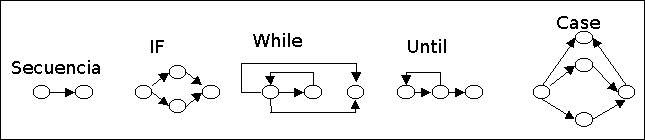
\includegraphics[scale=0.475]
	{control_flujo.png}}
	\caption{\label{fig:control_flujo} Grafos para las distintas estructuras de control.}
\end{figure}

\section{Complejidad ciclomática}

Una vez representado un algoritmo con grafos se puede hacer la siguiente medición:

\[
	M = E - N + 2P
\]

Donde $M$ es la complejidad. $E$ el numero de lados del grafo, $N$ el numero de nodos y $P$ el numero de componentes conexas.

Luego, uno puede clasificar las distintas posibilidades de complejidad en las siguientes categorías:

\begin{table}[h!]
\centering
\scalebox{1.3}{
\begin{tabular}{|l|l|lll}
\cline{1-2}
1-5:   & Facil de mantener   &  &  &  \\ \cline{1-2}
6-10:  & Dificil de mantener &  &  &  \\ \cline{1-2}
11-15: & Muy dificil         &  &  &  \\ \cline{1-2}
20+:   & Casi imposible      &  &  &  \\ \cline{1-2}
\end{tabular}}
\end{table}

\section{Metodología}

Usando Lizard\cite{1} podremos medir la complejidad ciclomática de cada método dentro de nuestras clases de Java.

\section{Resultados}
\begin{verbatim}
================================================
  NLOC    CCN   token  PARAM  length  location
------------------------------------------------
	16	5	180	0      20 Maze::generarNodos@35-54@.\Maze.java
	39	10	329	0      59 Maze::siguientesPasadas@79-137@.\Maze.java
	13	6	127	2      14 Maze::areNodesEquivalent@182-195@.\Maze.java
\end{verbatim}

Es el resultado del análisis de Lizard. A partir de esto podemos determinar que hay 2 métodos en el proyecto que serían `difícil de mantener'.

\section{Subrutinas largas}

Las rutinas `largas' tienen una mala reputación en el ambiente empresarial y en la programación orientada a objetos. Existe la idea de compartimentar al máximo los métodos de una clase llegando en algunos casos a lo absurdo. Con el objetivo de hacer más fácil de entender estas rutinas se puede llegar a tal punto donde hay recorrer varios métodos para lograr entender un `algoritmo'. Creo que esto no es siempre lo correcto, y se puede lograr el objetivo escribiendo la acción que se quiere realizar en un solo método, bien ordenado, e.g. Aprovechando los distintos scopes que se pueden hacer dentro de métodos en lenguajes como Java.

\section{Conclusión}

La rutina `siguientesPasadas' tiene un numero de complejidad ciclomática de 10, algunos lo considerarían cómo muy alto, para disminuir este numero se tratará de mejorar el grafo de flujo del método sin aumentar la cantidad de métodos necesarios para terminar la acción.

\begin{thebibliography}{1}
\bibitem{1} \href{http://www.lizard.ws/}{Lizard}

\end{thebibliography}


\end{document}
